\section{Analýza datasetu}
\label{sec:Chapter31}
Pro účely trénování našich konvolučních neuronových sítí máme dostupný dodaný dataset snímků LEGO modelu 42022 Hot Rod. Dataset tvoří synteticky vykreslené RGB obrázky ve formátu JPEG o velikosti $256\times256$ pixelů pro pravé a falešné snímky (syntetické snímky mají poloviční velikost $128\times128$). Barevná hloubka obrázků je 24 bitů (16 777 216 barev). Dataset je konstruován pro 11 vybraných klíčových bodů, kde každý klíčový bod chápeme jako svou vlastní klasifikační třídu. Pro každý klíčový bod máme dostupných 50 000 shluků informací, které jsou dostupny pro každou třídu klíčového bodu v CSV souboru. Mezi tyto informace patří:
\begin{enumerate}
  \item \textbf{Pravý snímek} -- $256\times256$ JPEG snímek se známou souřadnicí pro daný klíčový bod. Pravý snímek obsahuje daný model, či jeho část, a náhodné různorodé pozadí.
  \item \textbf{Falešný snímek} -- $256\times256$ JPEG snímek s potvrzeným nevyskytnutím daného klíčového bodu. Falešné snímky nabírají mnoha podob a nemusí vůbec obsahovat žádnou část daného modelu.
  \item \textbf{Syntetický snímek} -- $128\times128$ JPEG snímek, kde byl klíčový bod přetransformován do středu obrázku. K povšimnutí je, že tyto snímky obsahují model a černé pozadí.
  \item (x, y) souřadnice klíčového bodu na pravém snímku
  \item Rotace mezi pravým a syntetickým snímkem klíčového bodu, rotace má počátek v bodě pozice klíčového bodu
  \item Uniformní poměr měřítka mezi pravým a syntetickým snímkem klíčového bodu
\end{enumerate}

(x, y) souřadnice jsou v nenormalizované formě vyskytující se pro klíčový bod počínající od levého horního rohu v rozsahu od 0 do 255 hodnot s plovoucí desetinnou čárkou. Pro každý snímek dané třídy klíčového bodu, které budeme označovat celočíselně od 0 do 10, je dána pouze informace ohledně daného klíčového bodu. Na snímku se ve skutečnosti může vyskytovat více tříd klíčových bodů. Nevýhodou tohoto datasetu je avšak to, že pro tyto další třídy už v daném snímku nemáme žádné informace. Tento problém je následně adresován v implementační části této práce.



\begin{figure}[H]
\centering

% width is 0.86in corresponding to 150DPI for 128/128
\newcommand{\subfiguresize}{.15\textwidth}
\newcommand{\imagewidth}{0.86in}
\newcommand{\hspacesize}{.43in}

% Example of using minipage for an image block
\newcommand{\insertimage}[1]{%
  \begin{minipage}{\imagewidth}
    \centering
    \includegraphics[width=\imagewidth]{#1}
  \end{minipage}
}

% Row 1
\subfloat[snímek 0]{%
  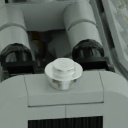
\includegraphics[width=\imagewidth]{Figures/sp_examples/sp00.jpg}%
  \label{fig:sp00}%
}\hspace{\hspacesize}%
\subfloat[snímek 1]{%
  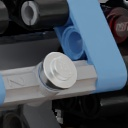
\includegraphics[width=\imagewidth]{Figures/sp_examples/sp01.jpg}%
  \label{fig:sp01}%
}\hspace{\hspacesize}%
\subfloat[snímek 2]{%
  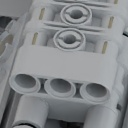
\includegraphics[width=\imagewidth]{Figures/sp_examples/sp02.jpg}%
  \label{fig:sp02}%
}

% Row 2
\subfloat[snímek 3]{%
  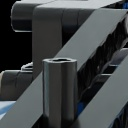
\includegraphics[width=\imagewidth]{Figures/sp_examples/sp03.jpg}%
  \label{fig:sp03}%
}\hspace{\hspacesize}%
\subfloat[snímek 4]{%
  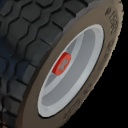
\includegraphics[width=\imagewidth]{Figures/sp_examples/sp04.jpg}%
  \label{fig:sp04}%
}\hspace{\hspacesize}%
\subfloat[snímek 5]{%
  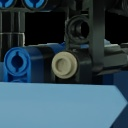
\includegraphics[width=\imagewidth]{Figures/sp_examples/sp05.jpg}%
  \label{fig:sp05}%
}

% Row 3
\subfloat[snímek 6]{%
  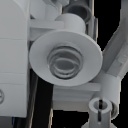
\includegraphics[width=\imagewidth]{Figures/sp_examples/sp06.jpg}%
  \label{fig:sp06}%
}\hspace{\hspacesize}%
\subfloat[snímek 7]{%
  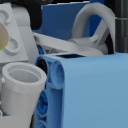
\includegraphics[width=\imagewidth]{Figures/sp_examples/sp07.jpg}%
  \label{fig:sp07}%
}\hspace{\hspacesize}%
\subfloat[snímek 8]{%
  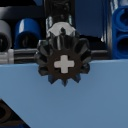
\includegraphics[width=\imagewidth]{Figures/sp_examples/sp08.jpg}%
  \label{fig:sp08}%
}

% Row 4
\subfloat[snímek 9]{%
  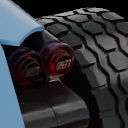
\includegraphics[width=\imagewidth]{Figures/sp_examples/sp09.jpg}%
  \label{fig:sp09}%
}\hspace{\hspacesize}%
\subfloat[snímek 10]{%
  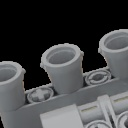
\includegraphics[width=\imagewidth]{Figures/sp_examples/sp10.jpg}%
  \label{fig:sp10}%
}\hspace{\hspacesize}%
\subfloat{%
  \hspace{\imagewidth}
}

\caption[Příklady syntetických snímků z datasetu]{Příklady syntetických snímků z datasetu, klíčový bod se nachází ve všech obrázcích uprostřed. Syntetické snímky viditelně obsahují černé pozadí, což je rozdílem oproti reálným snímkům. }
\label{fig:synthetic_images}
\end{figure}

Na obrázku \ref{fig:synthetic_images} je zřetelné, že se různé třídy klíčových bodů nacházejí i na vzájemně podobných nebo identických částech stavebnice modelu. Nejlepším příkladem může být klíčový bod 0 a klíčový bod 1. Klíčové body také i nabírají podobných tvarů, většinou kruhových. Tato povaha tříd klíčových bodů představuje jistou formu náročnosti pro modely strojového učení.

\endinput